\section{Создание конечно-элементной модели самолета схемы ``летающее крыло''}

В ходе работы были исследованы вопросы построения проектировочной модели самолета схемы ``летающее крыло'', а именно беспилотного летательного аппарата, проектируемого для целей разведки. Создание модели проводилось с помощью программного комплекса ``Conver'' (см. раздел \ref{sec:Conver})

\begin{figure}[ht]
\centering
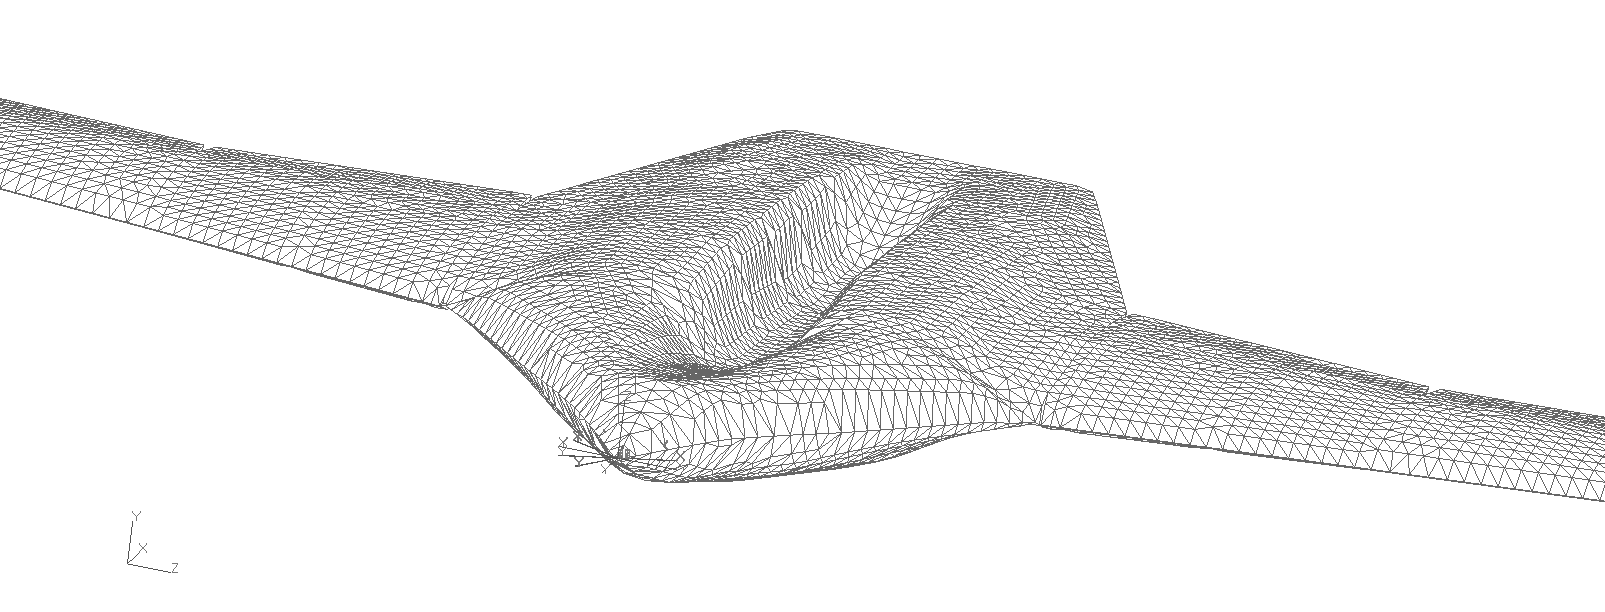
\includegraphics[width=0.6\textwidth]{BPLAfullModel}
\caption{МКЭ-модель БПЛА}
\label{fig:BPLAfullModel}
\end{figure}

\subsection{Подбор оптимального размера конечного элемента}

В целях обеспечения точности результатов необходимо понимать, как зависит НДС самолета от различных параметров. Было проведено исследование зависимости НДС самолета от максимального характерного размера конечных элементов, используемых в модели. 

С помощью комплекса ``Conver'' было построено 7 моделей самолета, отличающихся лишь размером конечного элемента. Путем расчета моделей были определены средние величины напряжений для стенок в наиболее напряженных отсеках (обозначены белым на  Рис.\ref{fig:WingRootPlain})

\begin{figure}[ht]
\centering
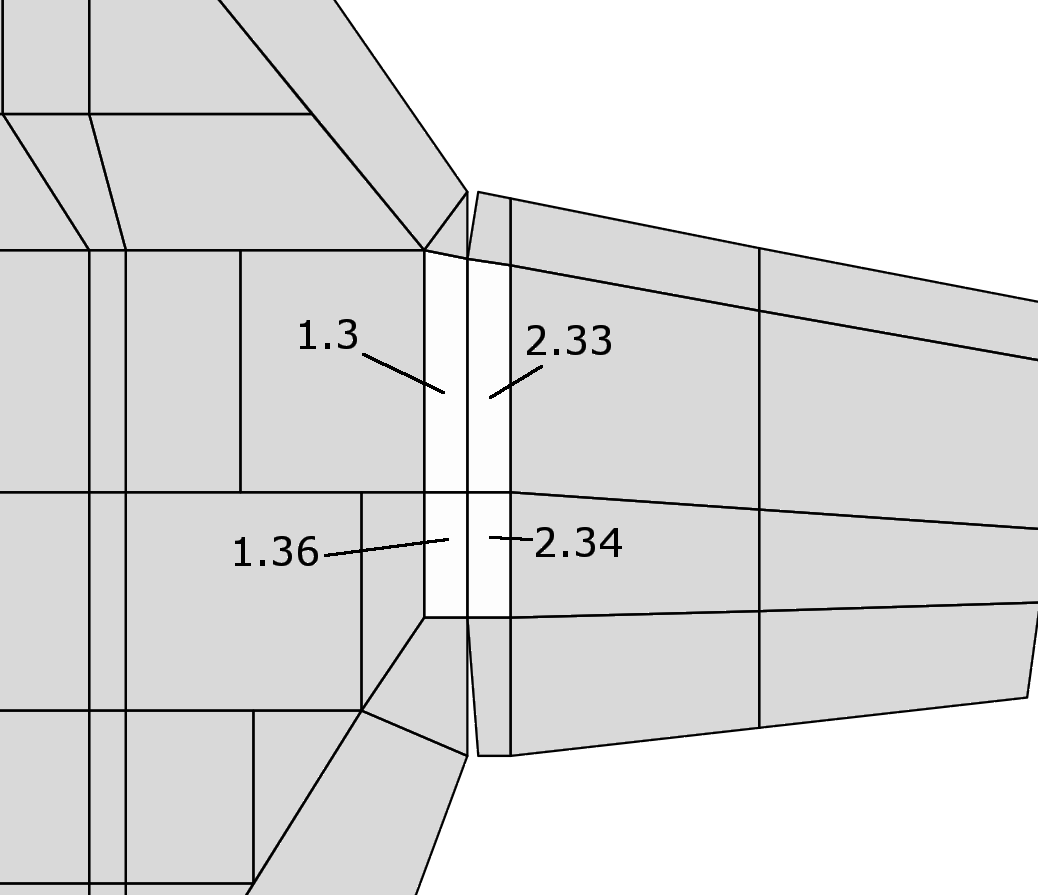
\includegraphics[width=0.6\textwidth]{RootOfWingWithSelectedPartsBW}
\caption{Стык правого крыла и фюзеляжа. Схематичное изображение вида сверху}
\label{fig:WingRootPlain}
\end{figure}




Была получена зависимость средних напряжений в этих отсеках от размера конечного элемента (Рис.\ref{fig:stressToDiscreteness})
\begin{figure}[ht]
\centering
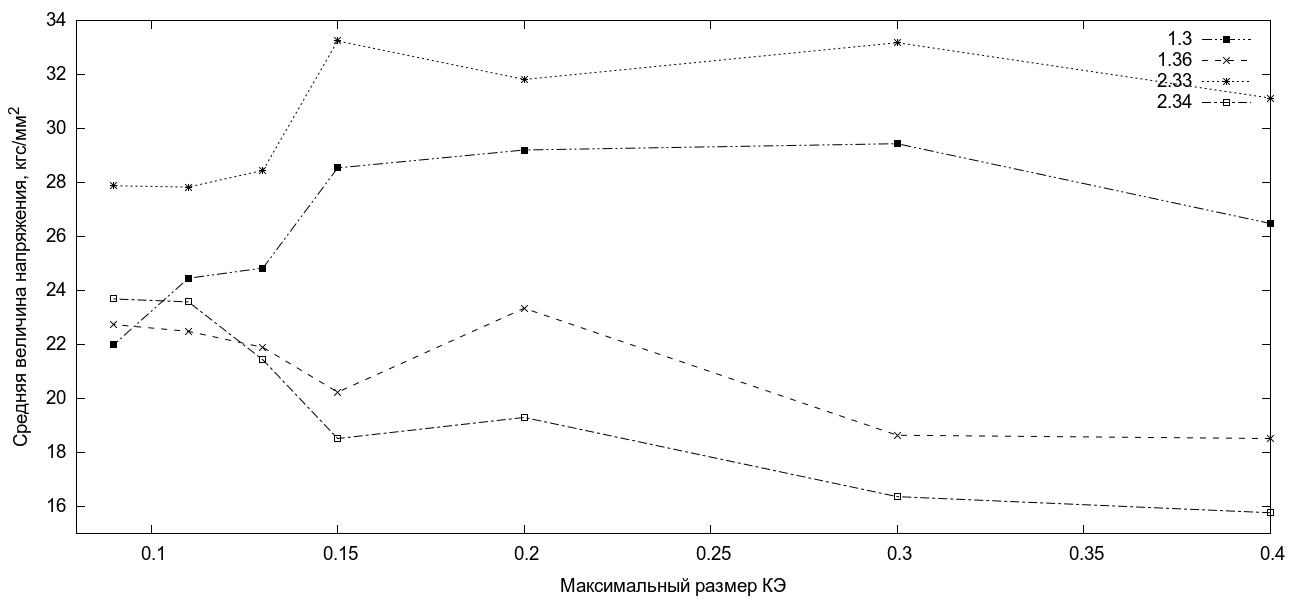
\includegraphics[width=0.8\textwidth]{StressToDiscretenessPlot}
\caption{Зависимость средних напряжений в отсеках от величины КЭ}
\label{fig:stressToDiscreteness}
\end{figure}

На основании полученных данных с учетом трудоемкости процесса расчета была определена оптимальная величина конечного элемента для дальнейшей работы над моделью, равная $0,11\text{м}$. 
%Ниже приведены картины НДС в месте стыка крыла с фюзеляжем при различных размерах конечного элемента. 